
\chapter{Rozwinięcie}

\section{Wprowadzenie do problemu}
Celem tej sekcji jest porównanie werfikacji modelowej i technik uczenia ze wzmocnieniem w konteście analizy 
modeli reprezentujących grę dla dwóch graczy. Przeanalizujemy znaną grę Kółko i Krzyżyk. Analiza będzie polegała na wykonaniu dwóch eksperymentów. Pierwszym w nich będzie 
zamodelowanie gry jako modelu logicznego. Zostanie to wykonane i opisane w formacie \textit{ Interpreted Systems Programming Language
(ISPL)}. Po zamodelowaniu będzie konstruowali formuły do sprawdzenia przez model checker \textbf{MCMAS} które będą 
odpowiadały problemowi znajdowania strategii wygrywającej dla jednego z graczy. Będziemy zaczynali w pewnej pozycji,
początkowej lub planszą częściowo zajętą. Pytanie o strategię wygrywającą, jest równoznaczne z pytaniem 
czy istnieje strategia dla danego gracza która niezależnie od strategii drugiego gracza doprowadzi go do zwycięstwa.
Będziemy również wykorzystywali algorytmy uczenia ze wzmocnieniem do nauki modelu gry. Następnie będziemy rozgrywali 
gry pomiędzy nauczonymi agentami (lub losowymi) i na podstawie serii wyników będzie stawiali hipotezę co do prawdziwości 
danej formuły.

Wybór gry kółko krzyżyk jako pierwszego środowiska jest umotywowany kilkoma aspektami. Gra kółko krzyżyk 
jest znane praktycznie każdemu i to sprawia, że próg wejścia jest niski. Co więcej każdy czytelnik zrozumie 
zagadnienie które będziemy omawiali. Sama gra pozostaje cały czas interesującym tematem badań i opracowań.
Możemy je znaleźć między innymi w ~\cite{Deepa}, ~\cite{Dalffa2019-DALTLU}, ~\cite{Fogel}.
Gra jest cały czas problemem otwartym. Dokładniej mówiąc, otwarty jest problem dowiedzenia czy istnieje 
strategię wygrywającą dla gier o różnym rozmiarze. Jak podaje ~\cite{beck2008combinatorial} nadal otwartym problemem 
pozostaje gra $5 \times 5 \times 5$. Dowiedzione zostałe strategie dla gier $3\times 3 \times 3$ oraz 
$4 \times 4 \times 4$. W obu tych grach istnieje strategia wygrywająca dla graczy rozpoczynających rozgrywkę.
Dla gry $5 \times 5 \times 5$ przypuszcza się, że będzie to gra remisowa.
\subsection{Model checker STV}
Narzędzi \textit{stv} ~\cite{jamroga_stv} to jedno z najlepszych dostępnych narzędzi do werfikacji modelowej.
Jego współautorem jest polski naukowiec prof. dr hab. Wojciech Jamroga. Zalicza się on do grona najlepszych ekspertów w tej 
tematyce. Jest on również autorem wielu publikacji z tego zakresu. Narzędzi \textit{stv} posłuży nam jako pewien punkt 
odniesienie w prównaniu z innymi narzędziami i metodami.
\subsection*{Model gry - STV}
Model gry zapisujemy w języku inspirowanym na języku \textit{ISPL}, nie mniej jest to 
autorski pomysł i różnicą się od \textit{ISPL}. Podobnie definiujemy agentów, formułę, 
inny jest mechanizm komunikacji pomiędzy agentami. Przedstawię najważniejsze fragmenty modelu 
wraz z ich opisem.

\begin{lstlisting}[language={}]
  Agent P1:
  LOCAL: [last_move_1,P1_00,P1_01,P1_02,P1_10,P1_11,P1_12,P1_20,P1_21,P1_22]
  ...
  INITIAL: [last_move_1:=0,P1_00:=0,P1_10:=0,P1_20:=0,P1_01:=0,P1_11:=0,P1_21:=0,P1_02:=0,P1_12:=0,P1_22:=0]
\end{lstlisting}
Definicja agenta rozpoczyna się jego nazwy, następnie definiowane są zmienne lokalne naszego 
agenta. Po definicji zmiennych lokalnych w sekcji \textit{INITIAL} ustawione są wartości 
początkowe zmienncyh lokalnych.
\begin{lstlisting}[language={}]
init idle
my_turn_1: idle -> start_turn
 play_local_1_00: start_turn[P1_00 == 0 ] -> end_turn[P1_00:=1, last_move_1:=0]
 play_local_1_01: start_turn[P1_01 == 0 ] -> end_turn[P1_01:=1, last_move_1:=1]
 ... 
 play_local_1_22: start_turn[P1_22 == 0 ] -> end_turn[P1_22:=1, last_move_1:=8]
\end{lstlisting}
Przechodzimy do akcji i stanów agenta. Określenie stanu początkowego `init idle` wskazuje,
na kto który stan będzie stanem początkowym. Składania języka jaki obowiązuje dla akcji 
jest taka :
\begin{lstlisting}[language={}]
akcja : stan poczatkowy[warunki] -> stan koncowy[aktualizacja]
\end{lstlisting}
Akcja przeprowadza agenta ze stanu w jakim się znajduje jeśli spełnia warunki 
do wykonania akcji. Po wykonaniu akcji zostaje wprowadzony nowy stan i zostają 
zaktualizowane zmienne lokalne. Dla każdego stanu w którym jest agent zdefiniowane 
są akcje które może wykonać. W naszym modelu agent wykonuje ruch jako jedną z $n^{2}$
akcji jeśli pole jest wolne. Po wykonaniu ruchu oznacza pole jako zajętę w swojej zmiennej
lokalnej.
\begin{lstlisting}[language={}]
shared[3] play_1_00[play]: end_turn[last_move_1==0] -> wait
shared[3] play_1_01[play]: end_turn[last_move_1==1] -> wait
...
shared[3] play_1_22[play]: end_turn[last_move_1==8] -> wait
... 
shared[3] play_2_00[play]: wait[P1_00 == 0] -> start_turn[P1_00:=2]
shared[3] play_2_01[play]: wait[P1_01 == 0] -> start_turn[P1_01:=2]
...
shared[3] play_2_22[play]: wait[P1_22 == 0] -> start_turn[P1_22:=2]
\end{lstlisting}
Następnym krokiem po wykonaniu ruchu przez Agenta jest przekazanie tej informacji do 
pozostałych agentów. Składania narzędzia \textit{STV} nie umożliwia wprowadzania zmienncyh 
globalnych, czy innego systemu współdzielenia pamięci pomiędzy kilku agentów. Do przekazywania 
informacji wykorzystany został mechanizm akcji współdzielonych, czyli takich które 
zostają wykonane przez pewną ilość agentów razem. W naszym przypadku liczbę agentów 
krzórzy wykonają akcje współdzieloną określamy przez \textit{shared[3]}. W tym 
kroku również mamy $n^{2}$ możliwych akcji, nie mniej tylko jedna z nich jest możliwa do podjęcia
, poprzez kontrolę wartości zmiennej \textit{last\_move\_x}. Akcje z prefiksem \textit{play\_1}
oznaczają, że ruch wykonał agent \textit{P1}, a akcje z prefiksem \textit{play\_1}
oznaczają, że akcje wykonał agent  \textit{P2}. Taki mechanizm pewnej synchronizacji 
umożliwia przekazywania pomiędzy agentami informacji o wykonanych ruchach i aktualizację 
ich pamięci lokalnej.

Model agenta \textit{P2} jest symetryczny do agenta \textit{P1}. Trzecim agentem 
będącym w środowisku jest agent \textit{Env}. Odpowiada on za kontrolę planszy.

\begin{lstlisting}[language={}]
shared[3] play_1_00[play]: turn_1[P3_00 == 0 && end ==0] -> 
check_score_1[round := round+1, P3_00:=1]
 ... 
shared[3] play_1_22[play]: turn_1[P3_22 == 0 && end ==0] -> 
check_score_1[round := round+1, P3_22:=1]
shared[3] play_2_00[play]: turn_2[P3_00 == 0 && end ==0] -> 
check_score_2[round := round+1, P3_00:=2]
...
shared[3] play_2_22[play]: turn_2[P3_22 == 0 && end ==0] -> 
check_score_2[round := round+1, P3_22:=2]
\end{lstlisting}

Agent \textit{Env} wykonuje akcje współdzielone z pozostałymi agentami które
służą do synchronizacji informacji. Agent ten kontroluje to co się dzieje na planszy, 
liczy wykonane ruchy i śledzi stan rozgrywki
Po każdy wykonanym ruchu dokonywana jest przez tego agenta kontrola stanu planszy 
w celu stwierdzenia przez niego czy wystąpił stan końcowy.
\begin{lstlisting}[language={}]
check_win_1 : check_score_1[(
(P3_00==1 && P3_01==1 && P3_02==1) || 
(P3_10==1 && P3_11==1 && P3_12==1) || 
(P3_20==1 && P3_21==1 && P3_22==1) ||
(P3_00==1 && P3_10==1 && P3_20==1) || 
(P3_01==1 && P3_11==1 && P3_21==1) || 
(P3_02==1 && P3_12==1 && P3_22==1) || 
(P3_00==1 && P3_11==1 && P3_22==1) || 
(P3_02==1 && P3_11==1 && P3_20==1))] -> 
end_game[P1_WIN:=1, end:=1]
\end{lstlisting}
Klasyczne sprawdzenia planszy odbywa się przez sprawdenie $n$ kolumn, $n$ wierszy i dwóch 
głównych przekątnych. Jeśli któryś z warunków zostanie spełniony to gra zostaje 
zakończona, a zwyciężca zostaje wskazany. Jeśli żaden z warunków niezostałby spełniony, 
a na planszy znajdowałyby się wolne pola, to do następnej tury zostałby dopusczony przeciwny gracz.
Jeśli na planszy nie znajdowałyby się wolne pola, to gra zostałby zakończona remisem.


Narzędzie \textit{STV} umożliwia wygenerowanie różnego rodzaju grafów. Poniżej pokazane zostaną 
gfrafy lokalne stanów/akcji dla gracza i środowiska.
\begin{figure}[h]
  \centering
  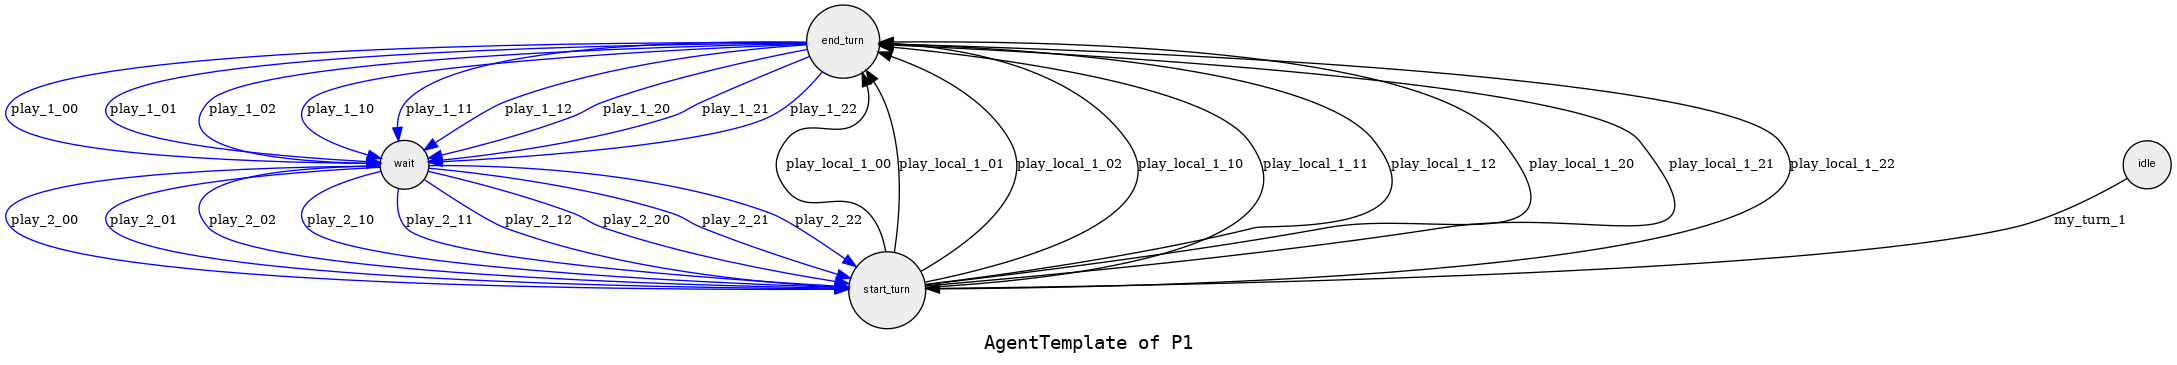
\includegraphics[width=\linewidth]{/home/pawblo/Desktop/future_mgr/text/figures/model-AgentTemplate_P1.png}
  \caption{Model agenta P1}
  \label{fig:enter-label}
\end{figure}

\begin{figure}[h]
  \centering
  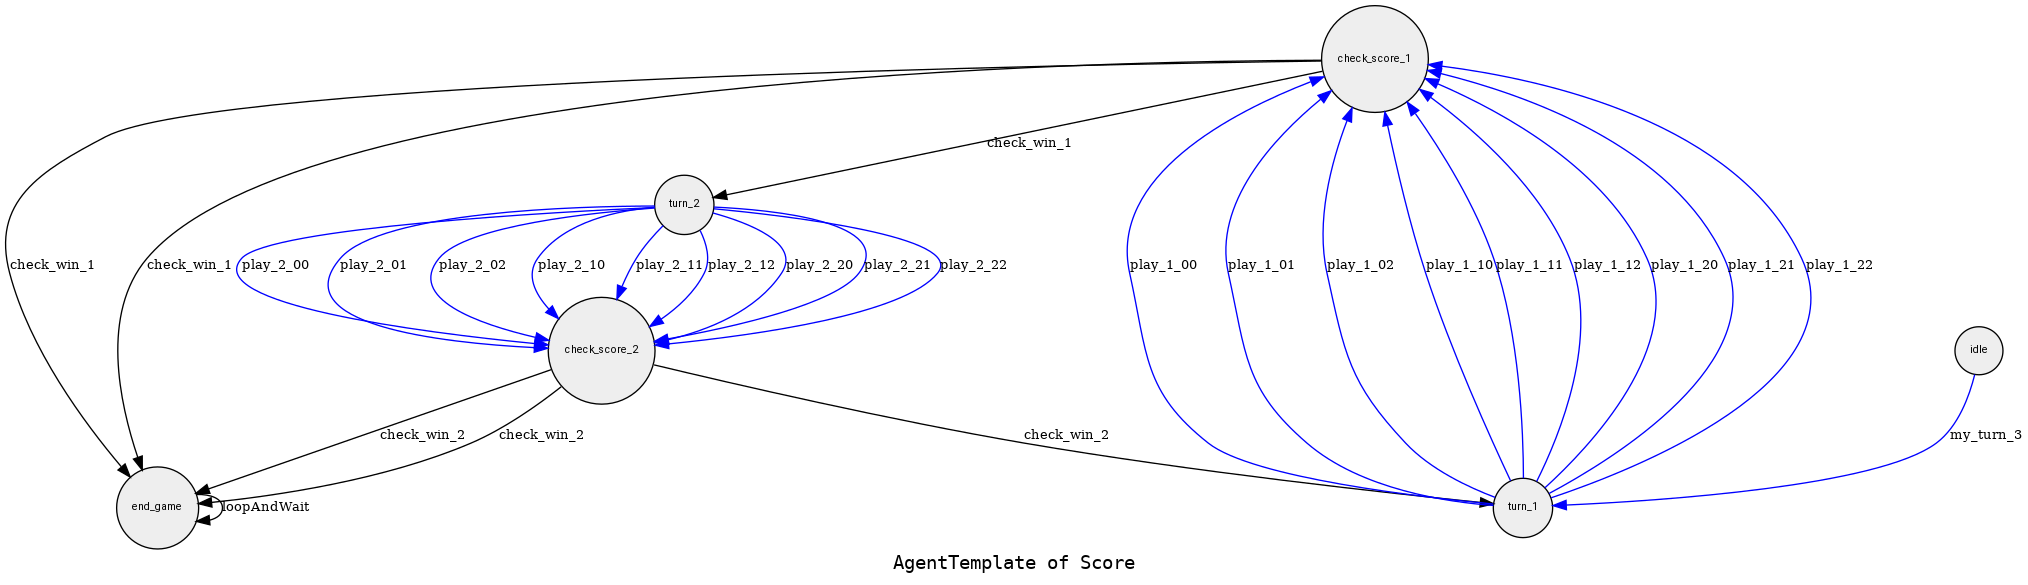
\includegraphics[width=\linewidth]{/home/pawblo/Desktop/future_mgr/text/figures/model-AgentTemplate_Score.png}
  \caption{Model agenta Env}
  \label{fig:enter-label}
\end{figure}


Na grfach możemy sprawdzić czy nasz zaprojektowany model działa tak jak zaplanowaliśmy. Jest to też ważna
funkcjonalnośc w kontekście debugowania i analizy działania modelu. W naszym kontekście możemy przeanalizować, 
czy nasz model zadziała dobrze w kontekście naszej gry w kółko i krzyżyk.



\subsection*{Eksperymenty - STV}
Analizę rozpoczniemy od analizy czasu jakiego potrzebuje \textit{stv} do werfikacji formuły. Pomiary prowadzimy dla gry kółko i krzyżyk 
na planszy o rozmiarach $3 \times 3$.
\begin{table}[h!]
  \centering
  \begin{tabular}{|c|c|c|c|}
  \hline
  Wolne pola & Czas wykonania (s)  \\
  \hline
  1 & 0.007 \\
  2 & 0.01 \\
  3 & 0.01 \\
  4 & 0.02 \\
  5 & 0.07 \\
  6 & 0.45 \\
  7 & 4.35 \\
  8 & 32 \\
  9 & 522\\
  \hline
  \end{tabular}
  \caption{Wyniki checkera stv dla gry na planszy 3x3}
  \label{table:mcmas_results}
  \end{table}
  Dla liczby wolnych pól powyżej $7$ czas werfikacji przekrasza $1s$, dla liczby wolnych $9$ czas wynosi około $10$ minut. Oznacza, to że do werfikacji czy istnieje strategia 
  wygrywająca dla danego gracza w grze kółko i krzyżyk na planszy $3 \times 3$ potrzebny jest czas $10$ minut. 





\section{Model gry}
Gra została zamodelowana w języku \textit{ISPL}. Jest to język który jest wykorzystywany przez narzędzie \textit{MCMAS}.
Przedstawimy kluczowe fragmenty modelu dla lepszego zrozumienia problemu i tego, w jakis posób działa werfikacka modelu.

% Gra została zamodelowana w formacie \textit{ISPL} który obsługuje \textit{MCMAS}. Przedstawione i omówione zostaną 
% kluczowe fragmenty modelu.
% \begin{lstlisting}[language={}]
%     Semantics=SingleAssignment;
%     \end{lstlisting}
%     \textbf{Description}: Specifies the semantics to be used in the model. `SingleAssignment` indicates that variables are assigned values only once per state transition.
    
%     \section{Environment Agent}
    \begin{lstlisting}[language={}]
    Agent Environment
      Obsvars:
        turn : {nought, cross};
        b11 : {x, o, b}; b12 : {x, o, b}; b13 : {x, o, b}; b14 : {x, o, b}; b15 : {x, o, b};
        b21 : {x, o, b}; ... 
       ...
      end Obsvars
    \end{lstlisting}
    Agent \textit{Environment} przechowuje dwa typy zmiennych. Agent posiada zmienną typu \textit{enumerate} czyli typu wyliczanego 
    która przechowuje informację o tym, który z graczy jest aktualnie na ruchu. Kolejne zmienne przechowują informację, o stanie 
    danego pola na planszy. Zmienna $bij$ przechowuje informację na temat pola w i-tym wierszu i -jtej kolumnie. Standard $ISPL$
    nie dopuszcza tablic, dlatego planszę musimy implementować za pomocą $n^{2}$ zmiennych. 
%       Actions = { }; 
%       Protocol: end Protocol
    \begin{lstlisting}[language={}]
      Evolution:
        turn=nought if turn=cross; turn=cross if turn=nought;
        b11 = o if turn = nought and Nought.Action = a11;
        b11 = x if turn = cross  and Cross.Action  = a11;
        ...
        b55 = o if turn = nought and Nought.Action = a44;
        b55 = x if turn = cross  and Cross.Action  = a44;
      end Evolution
    end Agent
     \end{lstlisting}
     Tury graczy zmieniją się na przemian. Agent \textit{Environment} pobiera od agentów graczy akcji jakie podjeli i aktualizuje 
     planszę gry jak i aktualną turę.
%     \textbf{Description}: The \texttt{Environment} agent maintains the game state, including the current turn (\texttt{turn}), and the state of each cell on the 4x4 board (\texttt{b11, b12, ... , b44}). The \texttt{Evolution} section updates the board and turn based on the actions of \texttt{Nought} and \texttt{Cross} agents.
    
    \begin{lstlisting}[language={}]
    Agent Nought
      Vars:
        null : boolean; -- for syntax reasons only
      end Vars
      Actions = {a11,a12,a13,a14,a15,a21,a22,a23,a24,
                a25,a31,a32,a33,a34,a35,a41,a42,a43,a44,a45,a51,a52,a53,a54,a55, };
      Protocol: 
        Environment.b11=b:{a11}; Environment.b12=b:{a12}; ... Environment.b15=b:{a15};
        ...
        Environment.b51=b:{a51};
      end Protocol
    end Agent
    \end{lstlisting}
    Powyżej znajduje się szkic implementacji agenta \textit{Nought}. Implementacja agenta \textit{Cross} jest symetryczna.
    Agent gracza ma do wyboru $n^{2}$ akcji typu $aij$. Każda taka akcja oznacza wykonanie ruchu i postawienie znaku w i-tym wierszu i j-tej kolumnie.
    Akcja taka może zostać wykonana jeśli pole na planszy jest puste.
    \begin{lstlisting}[language={}]
    Evaluation
      noughtwins if
        Environment.b11 = o and Environment.b12 = o and Environment.b13 = o or
        Environment.b14 = o and Environment.b15 = o or 
        ...
        Environment.b11 = o and Environment.b21 = o and Environment.b31 = o or
        Environment.b41 = o and Environment.b51
        ... 
        Environment.b11 = o and Environment.b22 = o and Environment.b33 and 
        Environment.b44 = o and Environment.b55 = o 
    end Evaluation
    \end{lstlisting}
    Sekcja ewaluacji zawiera w sobie warunki na zakończenie gry. Gracz wygrywa jeśli zapełni jedną kolumnę, wiersz 
    lub główną przekątną swoimi znakami. Warunków na zakończenie gry jest $2n+2$. Warunki zakończenia dla obu graczy 
    są takie same, różnią się tylko znakami.
    \begin{lstlisting}[language={}]
        InitStates
  Environment.b11=b and Environment.b12=b and Environment.b13=b 
  and Environment.b14=b and Environment.b15  = b 
  ...
  and Environment.turn = cross
end InitStates
\end{lstlisting}
Sekcja \textit{InitStates} zawiera w sobie stan początkowy modelu. Wszystka pola planszy są puste, a jeden z graczy 
jest graczem startowym.

\begin{lstlisting}[language={}]
Groups
  nought = {Nought}; cross = {Cross};
end Groups

Formulae
  <cross> F (crosswins and ! noughtwins); -- TRUE
  <nought> F (noughtwins and ! crosswins); -- FALSE
end Formulae
\end{lstlisting}
Ostatnim elementem modelu jest zadeklarowanie koalicjii agentów. W naszym przypadku koalcjia agentów składa się z jednego gracza.
Formuły jakie badamy, to formuły które sprawdzają czy dany gracz wygra. Zawsze sprawdzamy dwie formuły, 
aby uzyskać odpowiedź dla każdego z dwóch graczy.
\subsection{Badania}
Analizę wyników zaczniemy od analizy wyników uzyskanych za pomocą narzędzia \textit{MCMAS}.
\begin{table}[h!]
    \centering
    \begin{tabular}{|c|c|c|c|}
    \hline
    Rozmiar planszy & Czas wykonania (s) & Liczba osiągalnych stanów & Użycie pamięci BDD  \\
    \hline
     2x2 &  0.017 &41  & 8.8 MB  \\
     3x3 & 0.325 &6172 & 13.2 MB \\
     4x4&193.383 &1.01786e+07 & 168 MB \\
     5x5 & timeout & timeout & timeout \\
    \hline
    \end{tabular}
    \caption{Wyniki checkera MCMAS}
    \label{table:mcmas_results}
    \end{table}
    Badając rozgrywkę dla pustej planszy $n \times n$ już dla $n=5$ dostajemy timeout.
    Jest to związane wykładniczą eksplozją stanów jakie \textit{MCMAS} ma do przeanalizowania.
    Eksplozja stanów jest bezpośrednio związana z liczbą pól na jakich gracze mogą 
    dokonywać ruchów. Do dalszej analizy wykorzystamy częściowo zapełnioną planszę o rozmiarze 
    $5 \times 5 $ z pozostałymi 17 polami lub więcej.

    \begin{table}[h!]
      \centering
      \begin{tabular}{|c|c|c|c|}
      \hline
      Wolne pola & Czas wykonania (s) & Liczba osiągalnych stanów & Użycie pamięci BDD (MB)  \\
      \hline
      17 &  20.644 & 2.96682e+07  & 49.41   \\
       19 & 199.467 &2.5328e+08 & 125.25 \\
       20& 641.051 &7.4155e+08 & 273.37 \\
       21 & 1714 &2.1736e+09 & 575.39 \\
      \hline
      \end{tabular}
      \caption{Wyniki checkera MCMAS}
      \label{table:mcmas_results}
      \end{table}
      \begin{figure}[h]
        \centering
        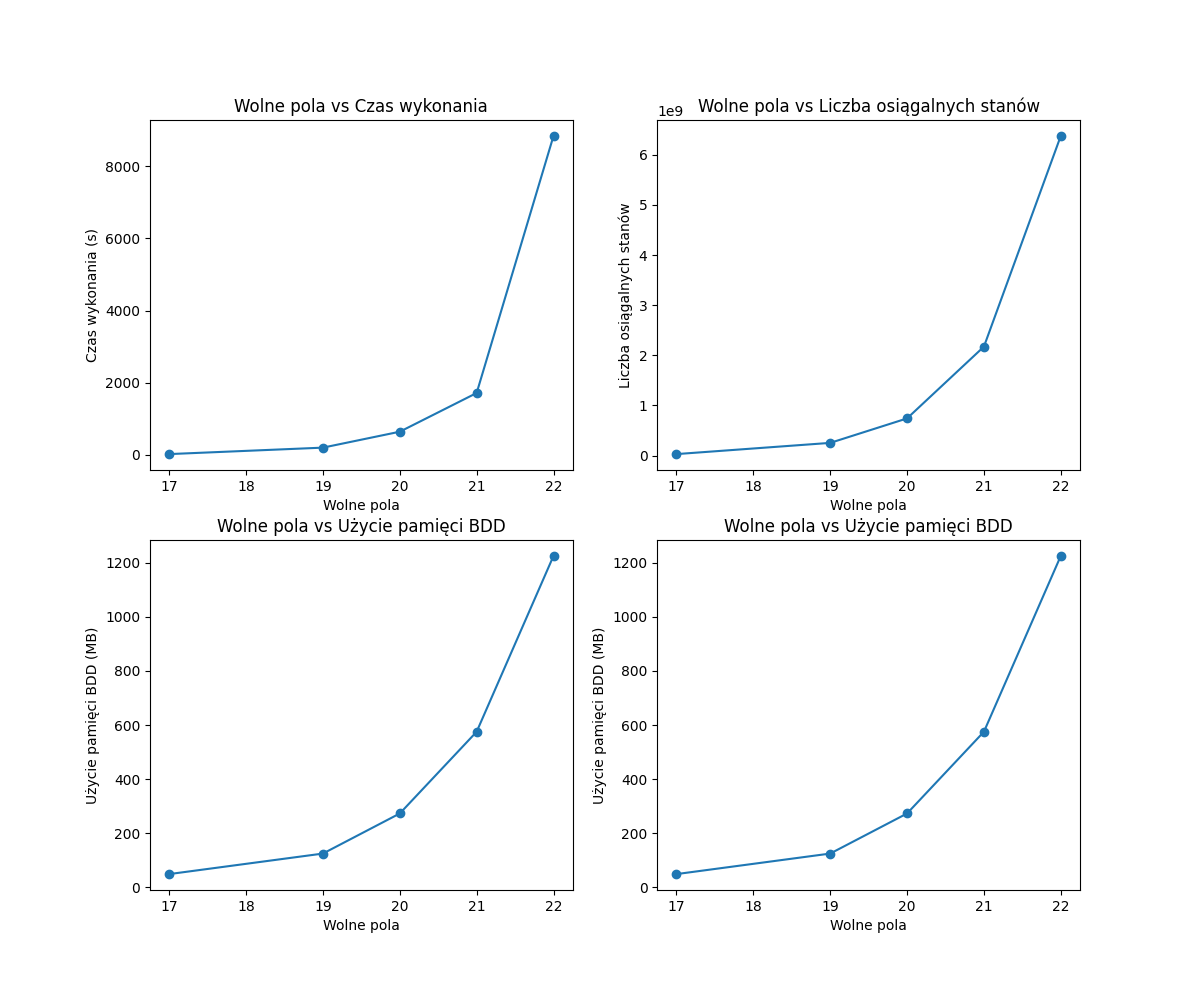
\includegraphics[width=\linewidth]{figures/wykres_wyniki_mcmas_1.png}
        \caption{Wykres wyników dla MCMAS}
        \label{fig:enter-label}
    \end{figure}


